\documentclass[12pt, a4paper, oneside]{ctexart}
\usepackage{amsmath, amsthm, amssymb, bm, color, framed, graphicx, hyperref, mathrsfs, mathtools, enumerate, tikz}
\usepackage{graphicx}
\usepackage{float}
\usepackage{subfig}

\usetikzlibrary{patterns}

\title{\textbf{Homework 4}}
\author{萃英学院\qquad 2022级\qquad 王一鑫}
\date{\today}
\linespread{1.5}
\newcounter{problemname}
\newenvironment{problem}{\begin{framed}\stepcounter{problemname}\par\noindent\textsc{Problem \arabic{problemname}. }}{\end{framed}\par}
\newenvironment{solution}{%
	\par\noindent\textsc{Solution. }\ignorespaces
}{%
	\hfill$\qed$\par
}
\newenvironment{note}{\par\noindent\textsc{Note of Problem \arabic{problemname}. }}{\\\par}

\begin{document}
	
	\maketitle
	
	\begin{problem}
		(Exercise 2.38)

        Find the shortest path from $S$ to each other vertex in the weighted graph of 
        Fig \ref{fig:WG}.

        \begin{figure}[H]
            \small
            \centering
            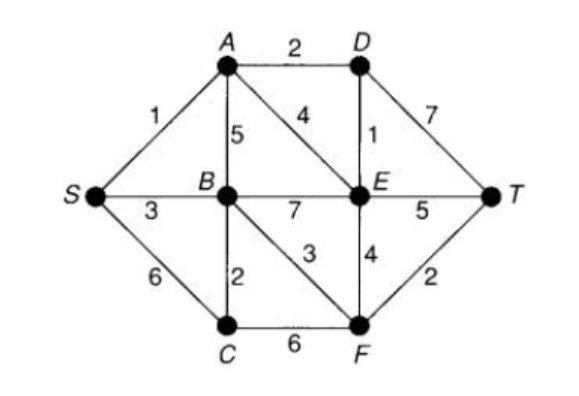
\includegraphics[width=0.5\columnwidth]{figure/fig1.png}
            \caption{Weighted Graph}
            \label{fig:WG}
        \end{figure}
	\end{problem}
	
	\begin{solution}
		
		Apply Dijkstra Algorithm to the weighted graph, we can label the graph as Fig \ref{fig:Dijkstra}.
		\begin{figure}[H]
            \small
            \centering
            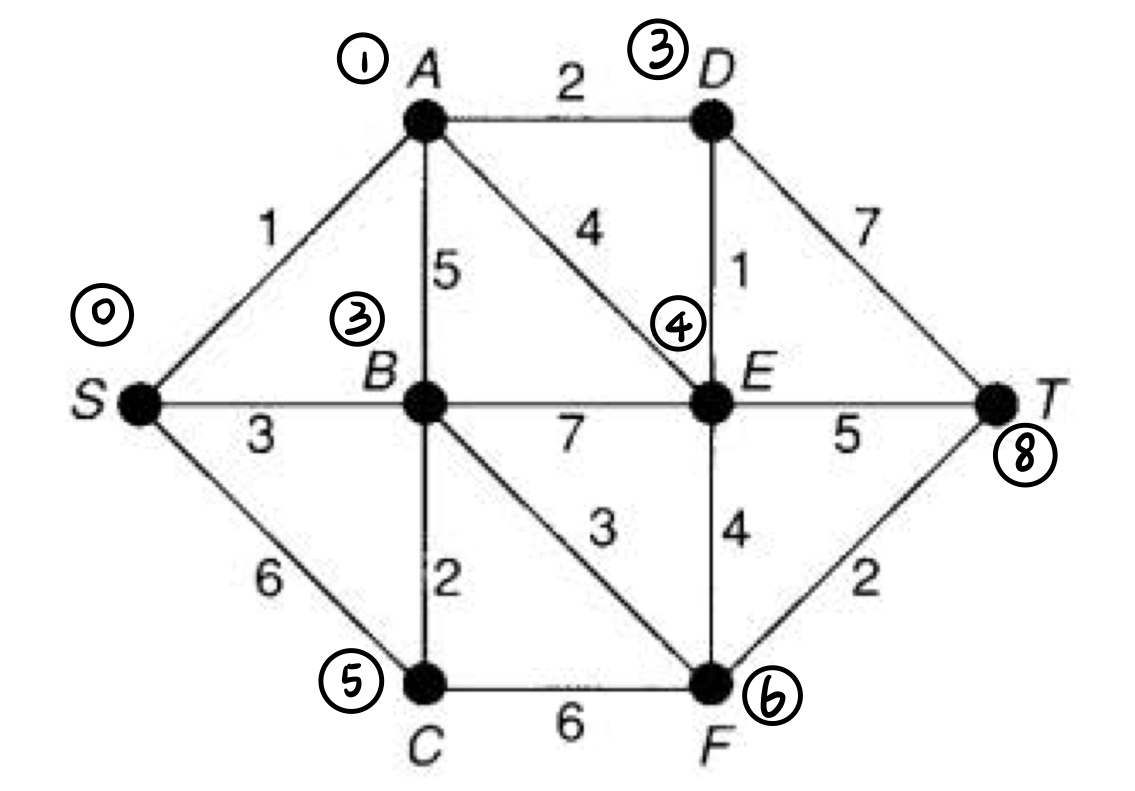
\includegraphics[width=0.5\columnwidth]{figure/Dijkstra.jpg}
            \caption{Labelled Graph}
            \label{fig:Dijkstra}
        \end{figure}
		
		From the labelled graph  we can see the shortest path from $S$ to each other vertex.
		\begin{enumerate}[(i)]
			\item $A$. It's $S \to A$, which length is $1$.
			\item $B$. It's $S \to B$, which length is $3$.
			\item $C$. It's $S \to B \to C$, which length is $5$.
			\item $D$. It's $S \to A \to D$, which length is $3$.
			\item $E$. It's $S \to A \to D \to E$, which length is $4$.
			\item $F$. It's $S \to B \to F$, which length is $6$.
			\item $T$. It's $S \to B \to F \to T$, which length is $8$.  
		\end{enumerate}
	\end{solution}
		

		
	
	\begin{problem}
		(Exercise 2.40)
        
        Find the longest path from $A$ to $G$ in the network of Fig \ref{fig:network}.

        \begin{figure}[H]
            \small
            \centering
            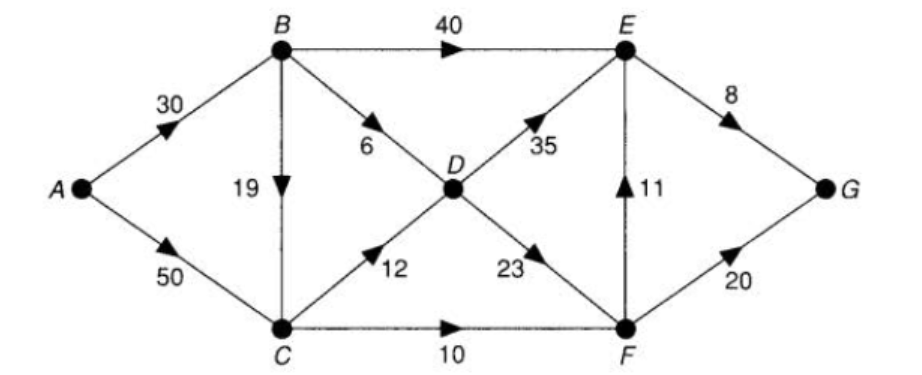
\includegraphics[width=0.75\columnwidth]{figure/fig2.png}
            \caption{Network}
            \label{fig:network}
        \end{figure}


	\end{problem}
	
	\begin{solution}
		
		We assign as follows:
		\begin{figure}[H]
            \small
            \centering
            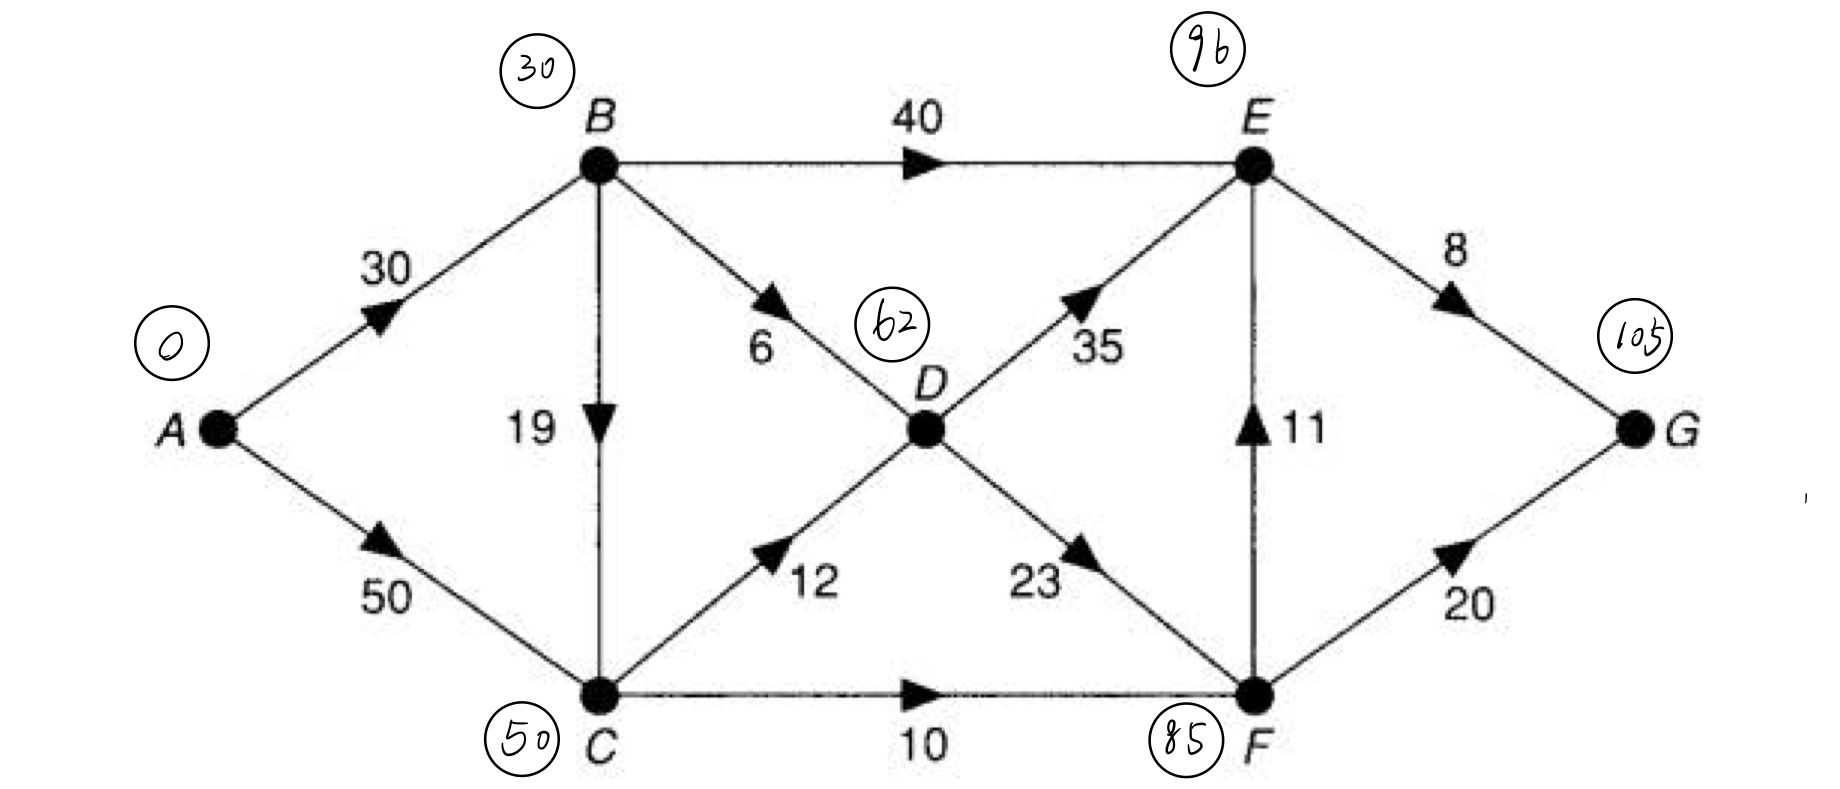
\includegraphics[width=0.75\columnwidth]{figure/LP.jpg}
            \caption{Labelled Graph}
            \label{fig:LP}
        \end{figure}
		to vertex $A$, the number $0$;

		to vertex $B$, the number $l(A) + 30$, that is, $30$;

		to vertex $C$, the largest of the numbers $l(A) + 50$ and $l(B) + 19$, that is, $50$;

		to vertex $D$, the largest of the numbers $l(B) + 6$ and $l(C) + 12$, that is, $62$;

		to vertex $F$, the largest of the numbers $l(C) + 10$ and $l(D) + 23$, that is, $85$;

		to vertex $E$, the largest of the numbers $l(F) + 11$, $l(B) + 40$ and $l(D) + 35$, that is, $96$;

		to vertex $G$, the largest of the numbers $l(E) + 8$ and $l(F) + 20$, that is, $105$.

		Then the longest path from $A$ to $G$ is $A \to C \to D \to F \to G$, and the length is $105$. The whole process is shown as Fig \ref{fig:LP}.

		
	\end{solution}
	
	\begin{problem}
		(Exercise 2.43)
		
        Find the Hamiltonian cycle of greatest weight in the graph of Fig \ref{fig:H}.

        \begin{figure}[H]
            \small
            \centering
            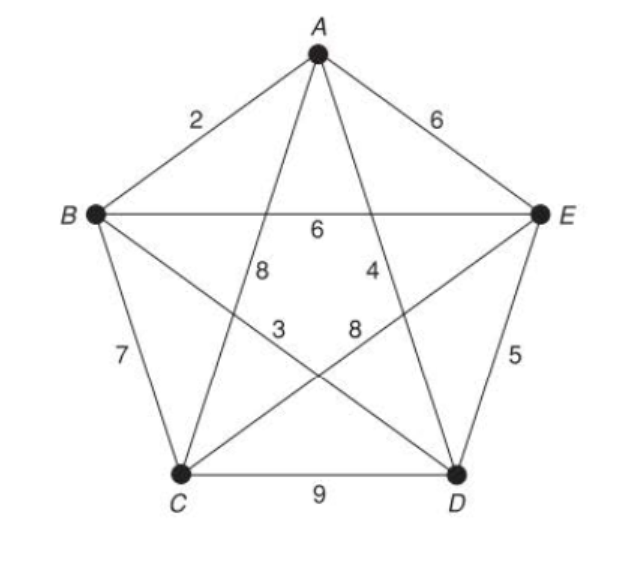
\includegraphics[width=0.5\columnwidth]{figure/fig3.png}
            \caption{Graph for problem 3}
            \label{fig:H}
        \end{figure}
	\end{problem}
	
	\begin{solution}
		
		There are $\dfrac{1}{2}\times 4! = 12$ possible cycles in the graph. After trying all
		the different Hamiltonian cycle, I find the cycle of greatest weight is 
		\[ A \to C \to D \to B \to E \to A\] and the weight is $32$.
		
		
	\end{solution}
	
	
	
	\begin{problem}
		(Exercise 2.45)

        Let $G$ be a connected graph with vertex-set $\{ v_1, v_2, \dots, v_n \}$, $m$ edges and $t$ triangles.

    \begin{itemize}
        \item[(i)] If $A$ is the adjacency matrix of $G$, prove that the number of walks of length 2 from $v_i$ to $v_j$ is the $ij$th entry of the matrix $A^2$. Deduce that $2m$ = the sum of the diagonal entries of $A^2$.
    
        \item[(ii)] Obtain a corresponding result for the number of walks of length 3 from $v_i$ to $v_j$, and deduce that $6t$ = the sum of the diagonal entries of $A^3$.
    \end{itemize}
		
	\end{problem}
	
	\begin{solution}
		
		\begin{enumerate}[(i)]
			\item Recall that if \( A = (a_{ij}) \) is the adjacency matrix of a graph \( G \) with \( n \) vertices \( v_1, v_2, \dots, v_n \), then \( A \) is an \( n \times n \) symmetric matrix, and \( a_{ij} \) is the number of edges joining \( v_i, v_j \) (0 or 1 for a simple graph), i.e., the number of walks of length 1 from \( v_i \) to \( v_j \). 
			Since \[(A^2)_{ij} = \sum_{k = 1}^{n}a_{ik}a_{kj}\]
			We know that \( (A^2)_{ij} \) is the number of walks of length \( 2 \) from \( v_i \) to \( v_j \) by definition.

			\( (A^2)_{ii} \) is the number of walks of length $2$ starting at \( v_i \) and finishing at \( v_i \). In a simple graph, we can only get back to the starting vertex in two steps by going to an adjacent vertex and back, and then we have the following equation.
			
			\[
			\begin{aligned}
    			(A^2)_{ii} &= a_{i1}a_{1i} + a_{i2}a_{2i} + \cdots + a_{in}a_{ni} \\
    			&= a_{i1}^2 + a_{i2}^2 + \cdots + a_{in}^2 \\
    			&= (0 \text{ or } 1) + (0 \text{ or } 1) + \cdots + (0 \text{ or } 1) \\
    			&= \text{the number of vertices } v_j \text{ adjacent to } v_i \\
    			&= \text{the degree of } v_i.
			\end{aligned}
			\]
			Sum up on both sides we get 
			\[ \text{tr}(A^2) = \sum_{i=1}^{n}\text{deg}(v_i) = 2m\]
			\item Similarly we have \[(A^3)_{ij} = \sum_{l=1}^{n}\sum_{k=1}^{n}a_{ik}a_{kl}a_{lj}\]
			Thus the $ij$th entry of the matrix $A^3$ is the number of walks of length $3$ from $v_i$ to $v_j$.

			\( (A^3)_{ii} \) is the number of walks of length $3$ starting at \( v_i \) and finishing at \( v_i \). In a simple graph, we can only get back to the starting vertex in three steps by going to two adjacent vertices and back.
			Thus, $(A^3)_{ii}$ is the number of triangles which contains the vertex $v_i$ without the order. For example, $v_iv_jv_k$ generates a triangle if $v_iv_jv_k$ are adjacent.
			When we count the number of triangles, since there are $6$ permutations for $v_iv_jv_k$, every triangles will be counted $6$ times. Therefore
			\[\text{tr}(A^3) = 6t\]

		\end{enumerate}

	\end{solution}


	\begin{problem}
		(Exercise 2.46)

        \begin{itemize}
            \item[(i)] Prove that, if two distinct cycles of a graph $G$ each contain an edge $e$, then $G$ has a cycle that does not contain $e$.
            \item[(ii)] Prove a similar result with `cycles' replaced by `cutsets'.
        \end{itemize}
		% \begin{figure}[h]
	
		% 	\begin{minipage}{0.32\linewidth}
		% 		\vspace{3pt}
				
		% 		\centerline{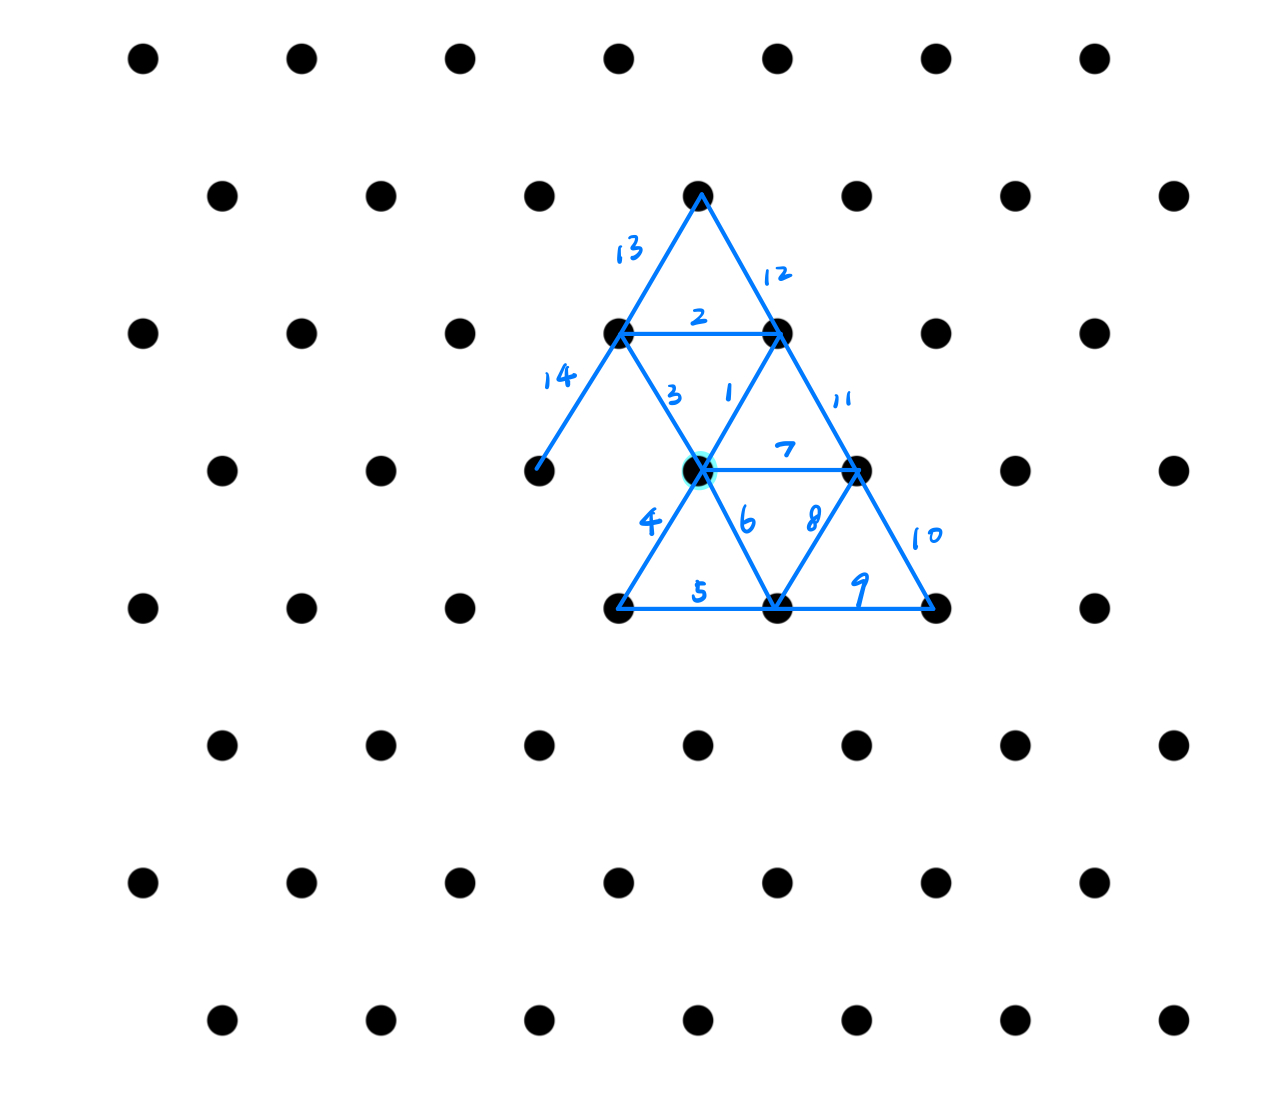
\includegraphics[width=\textwidth]{figure/fig6.png}}
			
		% 		\centerline{Step 1}
		% 	\end{minipage}
		% 	\begin{minipage}{0.32\linewidth}
		% 		\vspace{3pt}
		% 		\centerline{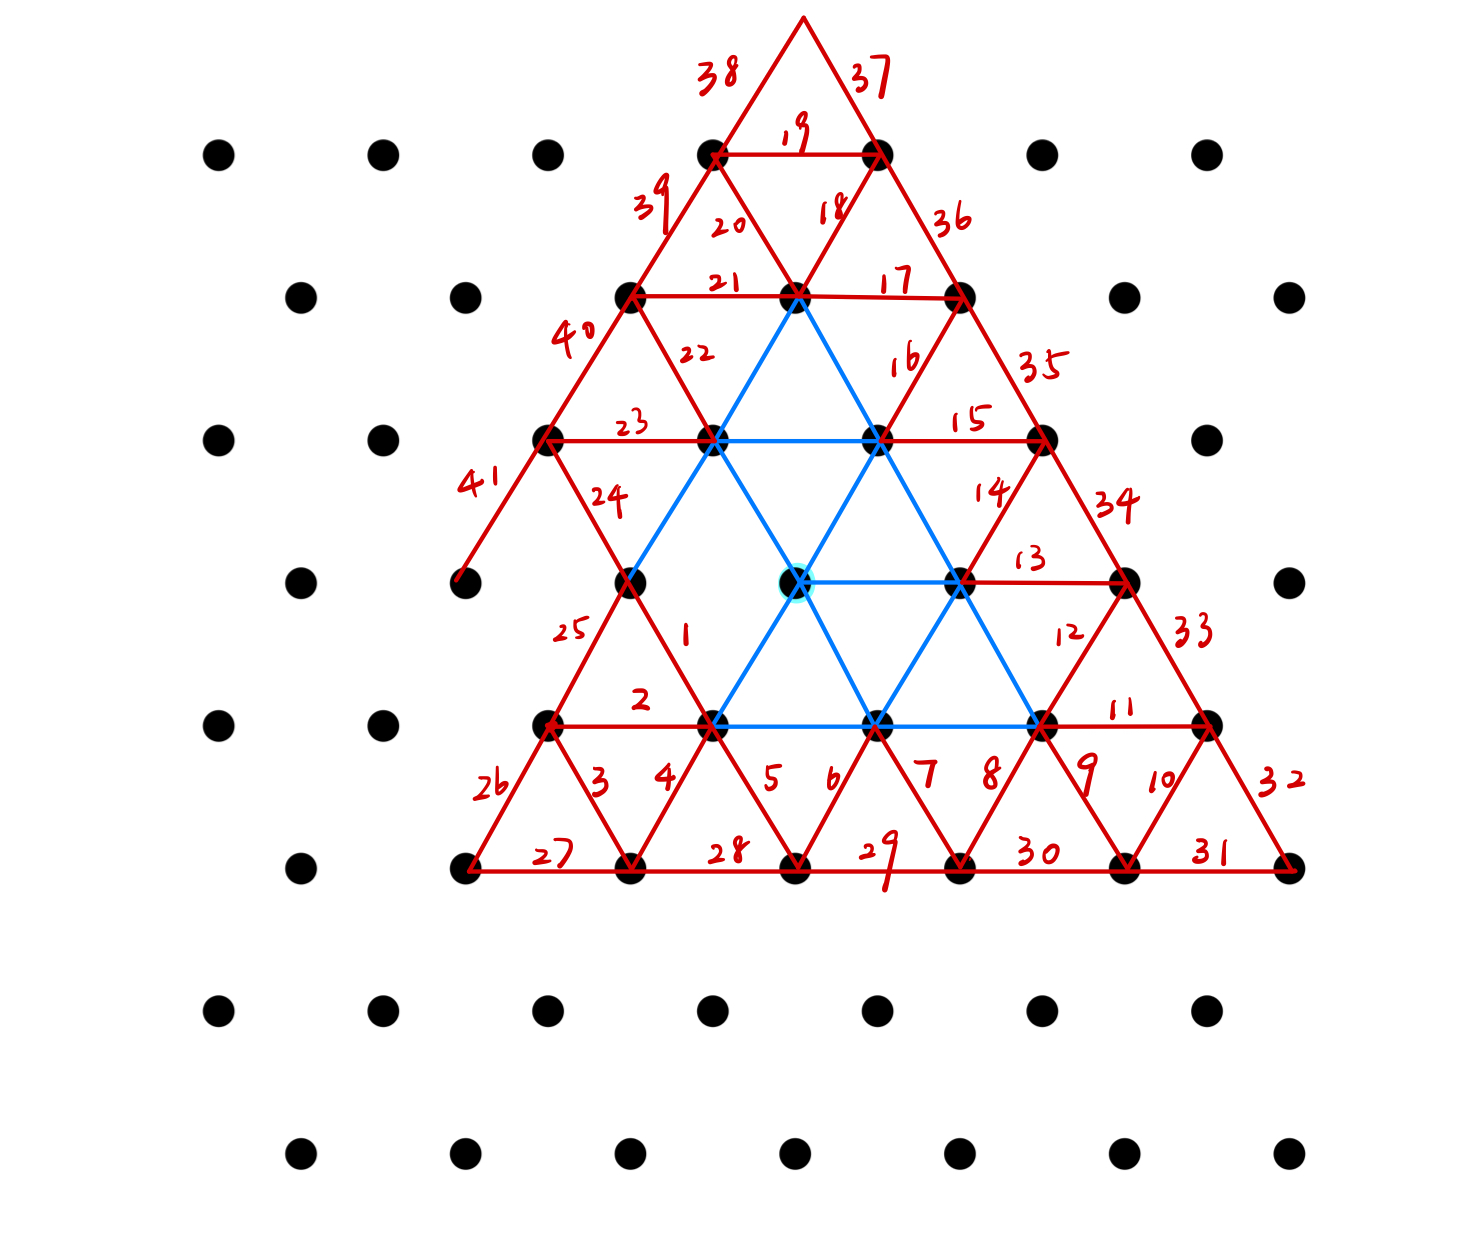
\includegraphics[width=\textwidth]{figure/fig7.png}}
			 
		% 		\centerline{Step 2}
		% 	\end{minipage}
		% 	\begin{minipage}{0.32\linewidth}
		% 		\vspace{3pt}
		% 		\centerline{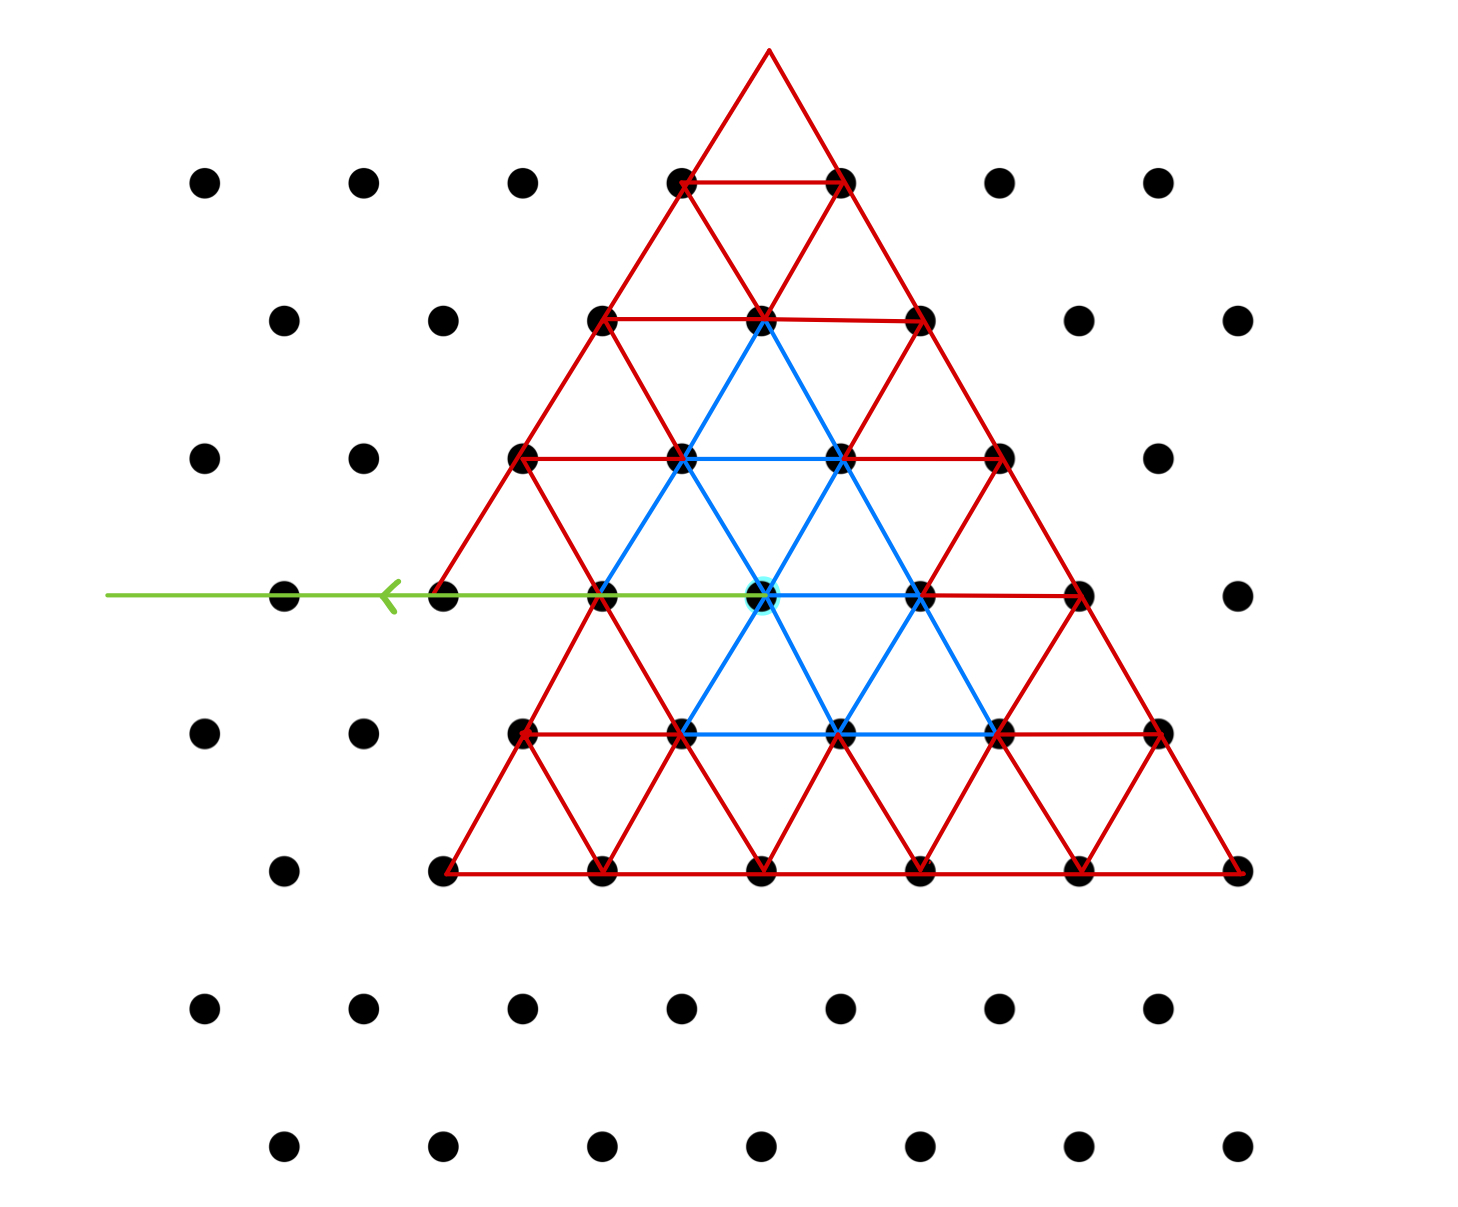
\includegraphics[width=\textwidth]{figure/fig8.png}}
			 
		% 		\centerline{Step 3}
		% 	\end{minipage}
		% 	\caption{Construction of Euler trail}
		% 	\label{fig:Construction}
		% \end{figure}
		
    \end{problem}

	\begin{solution}
        
		\begin{enumerate}[(i)]
			\item Given a graph $G = R \cup B$ composed of two simple cycles  
			$R$ and $B$, we can observe the behavior locally at each vertex. Each vertex will fall into one of the following five cases shown as Fig \ref{fig:5C}.
			\begin{figure}[H]
				\small
				\centering
				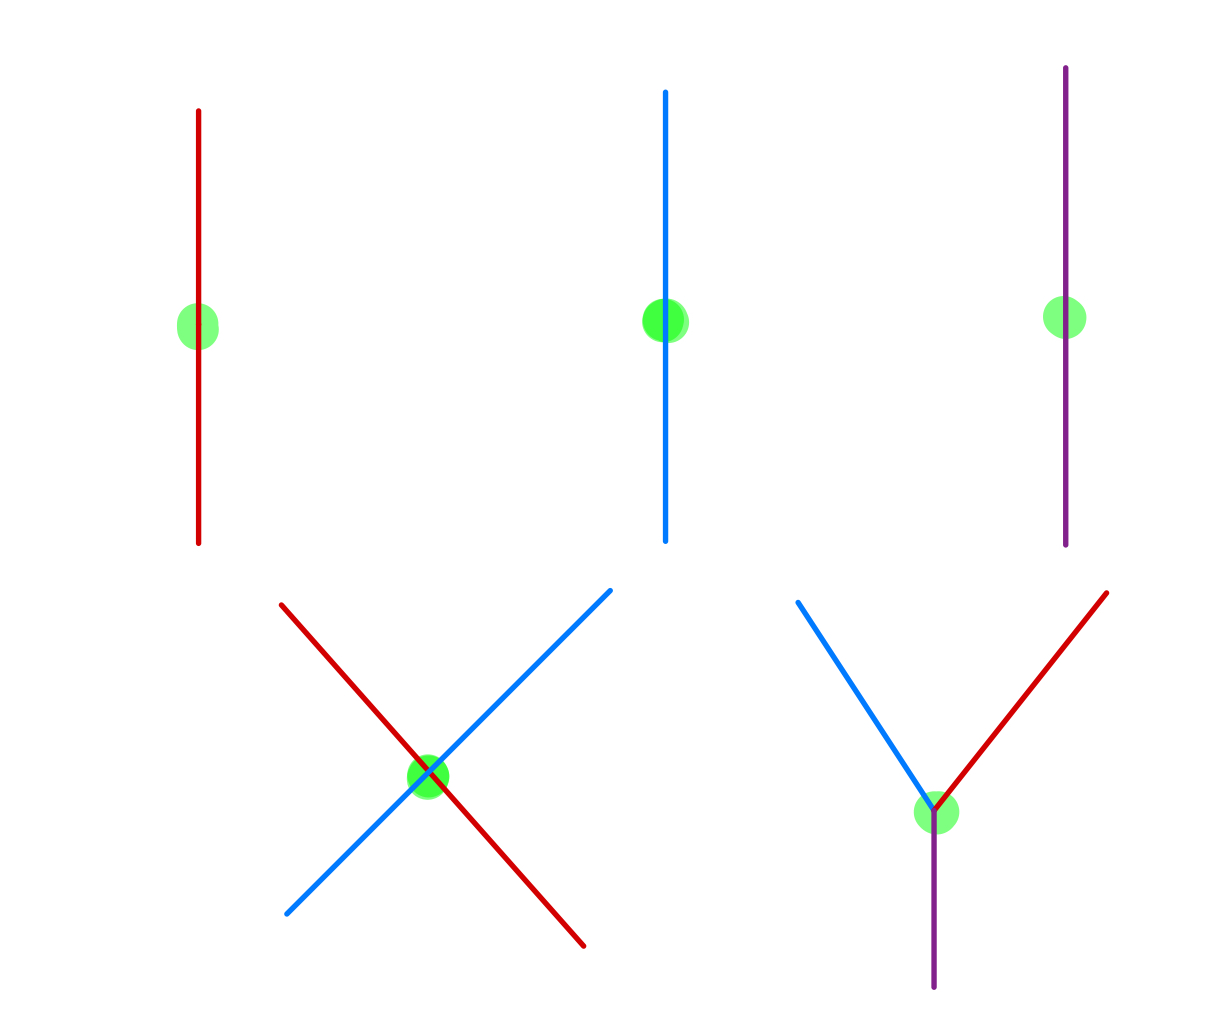
\includegraphics[width=0.5\columnwidth]{figure/5C.jpg}
				\caption{5 Cases}
				\label{fig:5C}
			\end{figure}

			where red edges belong to $R$ and blue edges belong to $B$, the purple ones are shared.

			We're given that a purple edge  $e$ exists and that  $R \neq B$. Modify $G$ by deleting all purple edges, which includes  
			$e$. W're left with a non-empty graph since not all edges are shared. And in fact, by observing the effect on the above illustrated cases, we see that all vertices now have \textbf{even} degree.
			Hence, some connected component of our modified graph contains an Eulerian cycle. And furthermore, an Eulerian cycle trivially contains a simple cycle. Since we removed  $e$
 			in the first step, we've found a simple cycle in  $G$ not containing  $e$.
			\item Suppose that there are two cutsets $(S_1, T_1)$ and $(S_2, T_2)$ of $G$, then WLOG we assume vertices $u \in S_1\cap S_2$
			and $v \in T_1\cap T_2$. Thus $e = uv$ is contained in both cutsets.

			Now if $S_1\cap T_2\neq\emptyset$, then we claim that $((S_1\cap T_2), G \setminus (S_1\cap T_2))$ is a cutset.
			In fact, for any vertex $w \in S_1 \cap T_2$, $w$ disconnects with any vertex in $S_2$ or $T_1$, which is also in 
			$G \setminus (S_1\cap T_2)$.

			Furthermore, since both $u$ and $v$ are not in $S_1\cap T_2$, $e\notin (S_1\cap T_2)$. The statement holds true for
			$S_2 \cap T_1$, and $S_1\cap T_2$ and $S_2 \cap T_1$ can not both be empty. Therefore, $((S_1\cap T_2), G \setminus (S_1\cap T_2))$ is a cutset that
			does not contain $e$.
		\end{enumerate}

    \end{solution}
		

	\begin{problem}
		(Exercise 2.47)

        \begin{itemize}
            \item[(i)] Prove that, if $C$ is a cycle and $C^*$ is a cutset of a connected graph $G$, then $C$ and $C^*$ have an even number of edges in common.
            \item[(ii)] Prove that, if $S$ is any set of edges of $G$ with an even number of edges in common with each cutset of $G$, then $S$ can be split into edge-disjoint cycles.
        \end{itemize}

    \end{problem}

	\begin{solution}
		
		\begin{enumerate}[(i)]
			\item Let \( U \) and \( W \) be the connected disjoint components of \( G - C^* \). 
			Then each of the vertices that \( C \) passes through is either in \( U \) or in \( W \). 
			We claim that an edge \( \{v_i, v_{i+1}\} \) is common to \( C \) and \( C^* \) if and only if \( v_i \in U \) 
			and \( v_{i+1} \in W \), or \( v_i \in W \) and \( v_{i+1} \in U \). 
			In fact, if not, then after removing \( \{v_i, v_{i+1}\} \) from \( C^* \) (i.e., `putting back' this edge into \( G \)) 
			the resulting graph is still disconnected, contradicting the minimality of \( C^* \). 
			Therefore the number of edges common to \( C \) and \( C^* \) is exactly equal to the number of times \( C \) traverses from \( U \) to \( W \). 
			Since \( C \) is a cycle, it returns to where it has started from, and this number therefore has to be even.
			\item Let \( G' \) be the graph obtained from \( G \) by removing all edges of \( G \) that are not in \( S \). 
			Then \( S \) can be split into edge-disjoint cycles if and only if each of its components is Eulerian. 
			This is equivalent to each vertex of \( G' \) having an even degree.
			
			Assume \( S \) cannot be split into edge-disjoint cycles. By the above, some vertex \( v \) of \( G' \) has an odd degree. 
			All vertices of \( G \) incident with \( v \) form a cutset, denoted as \( C^* \), of \( G \). 
			The edges common to \( S \) and \( C^* \) are exactly the edges in \( S \) incident to \( v \). 
			Their number is equal to the degree of \( v \) in \( G' \), and therefore odd, a contradiction.
			
		\end{enumerate}
		

		% \begin{figure}[H]
		% 	\small
		% 	\centering
		% 	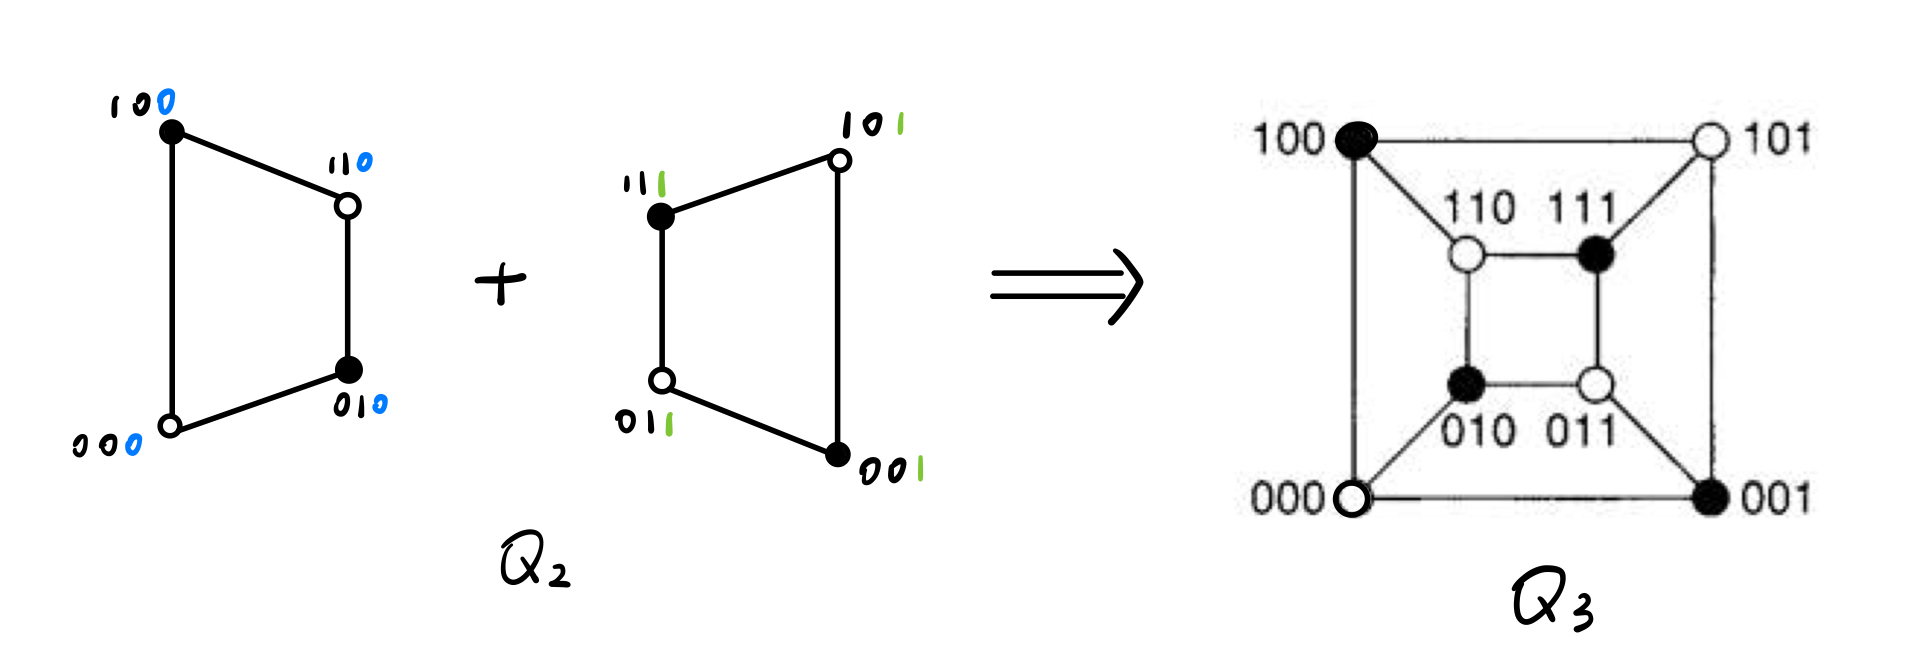
\includegraphics[width=0.75\columnwidth]{figure/fig9.png}
		% 	\caption{Example}
		% 	\label{fig:Q}
		% \end{figure}
		
	\end{solution}


	\begin{problem}
		(Exercise 2.52)

        Prove that the Petersen graph is non-Hamiltonian.

	\end{problem}

	\begin{solution}

		The Petersen graph has $10$ vertices. If it has a Hamilton Cycle, it must go through each vertex. 
		So then we can assume first that it is $C_{10}$ which has $10$ vertices and $10$ edges. Now, since Petersen graph has $15$
 		edges, we should add $5$ more edges to this cycle. 

		We discuss in different cases:
		\begin{enumerate}[(i)]
			\item \textbf{Case 1}: If each edge joins vertices opposite on $C$, then there is a $4$ cycle.
			\item \textbf{Case 2}: There exists an edge $e$ joins vertices at distance $4$ along $C$. Notice that no edge incident
			to a vertex opposite an endpoint of $e$ on $C$ can be added without creating a cycle with at most four vertices. Fig \ref{fig:Cases} shows an example.
			\item \textbf{Case 3}: otherwise. There must exists a $3$ cycle or $4$ cycle.
		\end{enumerate}

   		Since Petersen graph has no $3$ cycle or $4$ cycle. Therefore, the Petersen graph is non-Hamiltonian.
		\begin{figure}[h]
			\centering
			\begin{minipage}{0.45\linewidth}
				\vspace{3pt}
				
				\centerline{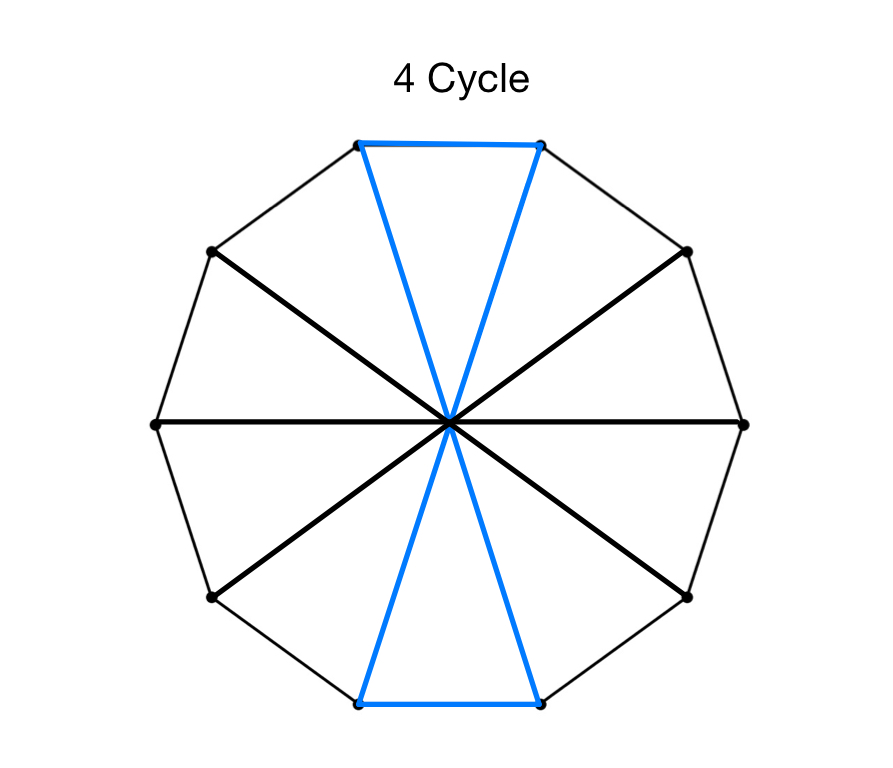
\includegraphics[width=\textwidth]{figure/C1.jpg}}
			
				\centerline{Case 1}
			\end{minipage}
			\begin{minipage}{0.38 \linewidth}
				\vspace{3pt}
				\centerline{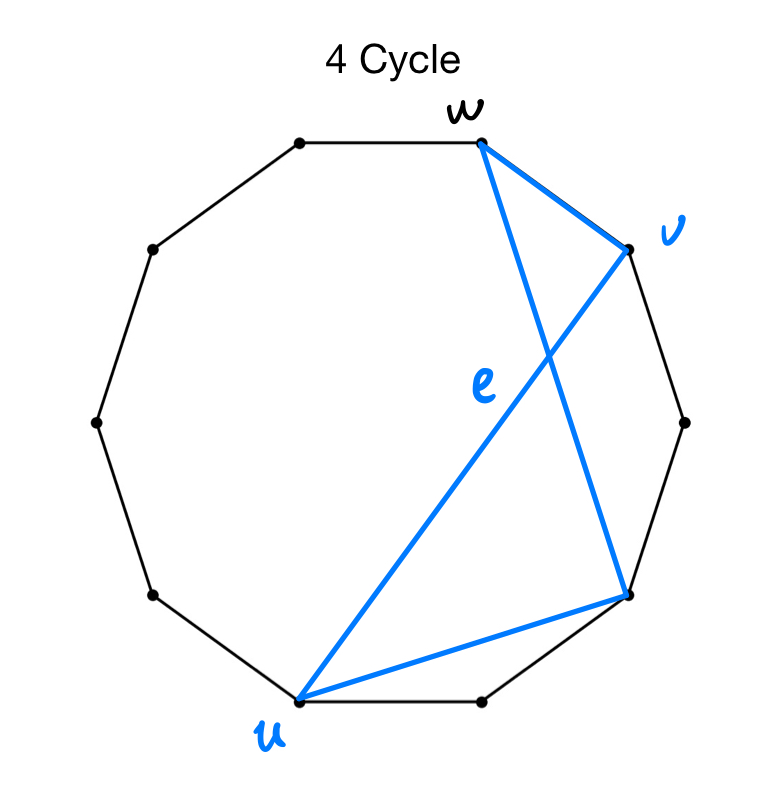
\includegraphics[width=\textwidth]{figure/C2.jpg}}
			 
				\centerline{Case 2}
			\end{minipage}
			\caption{Different Cases}
			\label{fig:Cases}
		\end{figure}

	\end{solution}

	
\end{document}


